% tikzpic.teP
\documentclass[crop,tikz]{standalone}% 'crop' is the default for v1.0, before it was 'preview'

%Packages
\usepackage{xcolor}
\usepackage{bm}
\usepackage{amsmath}
\usepackage{marvosym}

%tikz libraries}}
\usetikzlibrary{arrows.meta}
\usetikzlibrary{shapes.geometric}
% \tikzset{custom={latex[length=2in,width=2mm]}}

%Colors
\definecolor{recovery}{RGB}{27,158,119}
\definecolor{infection}{RGB}{217,95,2}
\definecolor{intervention}{RGB}{117,112,179}
\definecolor{susceptible}{RGB}{231,41,138}

\makeatletter
\tikzset{circle split part fill/.style  args={#1,#2,#3}{%
    alias=tmp@name, % Jake's idea !!
    postaction={%
      insert path={
        \pgfextra{%
          \pgfpointdiff{\pgfpointanchor{\pgf@node@name}{center}}%
          {\pgfpointanchor{\pgf@node@name}{north}}%
          \pgfmathsetmacro\scale{1}
          \pgfmathsetmacro\insiderad{\pgf@y*\scale}
          \fill[#1] (\pgf@node@name.base) ([yshift=-\pgflinewidth]\pgf@node@name.north) arc
          (90:210:\insiderad-\pgflinewidth)--(\pgf@node@name.center)--cycle;
          \fill[#2] (\pgf@node@name.base) ([yshift=-\pgflinewidth]\pgf@node@name.north)  arc
          (90:-30:\insiderad-\pgflinewidth)--(\pgf@node@name.center)--cycle; 
          \fill[#3] (\pgf@node@name.base) ([yshift=\pgflinewidth]\pgf@node@name.south)  arc
          (-90:-30:\insiderad-\pgflinewidth)--(\pgf@node@name.center)--cycle; 
          \fill[#3] (\pgf@node@name.base) ([yshift=\pgflinewidth]\pgf@node@name.south)  arc
          (270:210:\insiderad-\pgflinewidth)--(\pgf@node@name.center)--cycle;            %  \end{scope}
        }}}}}
 \makeatother

% Formatting macros:
\tikzstyle{node}=[minimum size= .5in,circle, draw]
\tikzset{intervened node fill/.style  args={#1,#2}{node,circle split part fill={#1,#2}}}
\tikzstyle{edge}=[minimum size = .5in, diamond, draw]

\tikzstyle{intervention}=[fill = intervention,text = white]
\tikzstyle{contact}=[fill = infection, text = white]
\tikzstyle{recovery}=[fill = recovery,text = white]
\tikzstyle{custom}=[-{Latex[scale=1,length=1.5mm,width=1.5mm]},color=black!40!white]

\renewcommand{\Leftscissors}{\Huge X}

\begin{document}


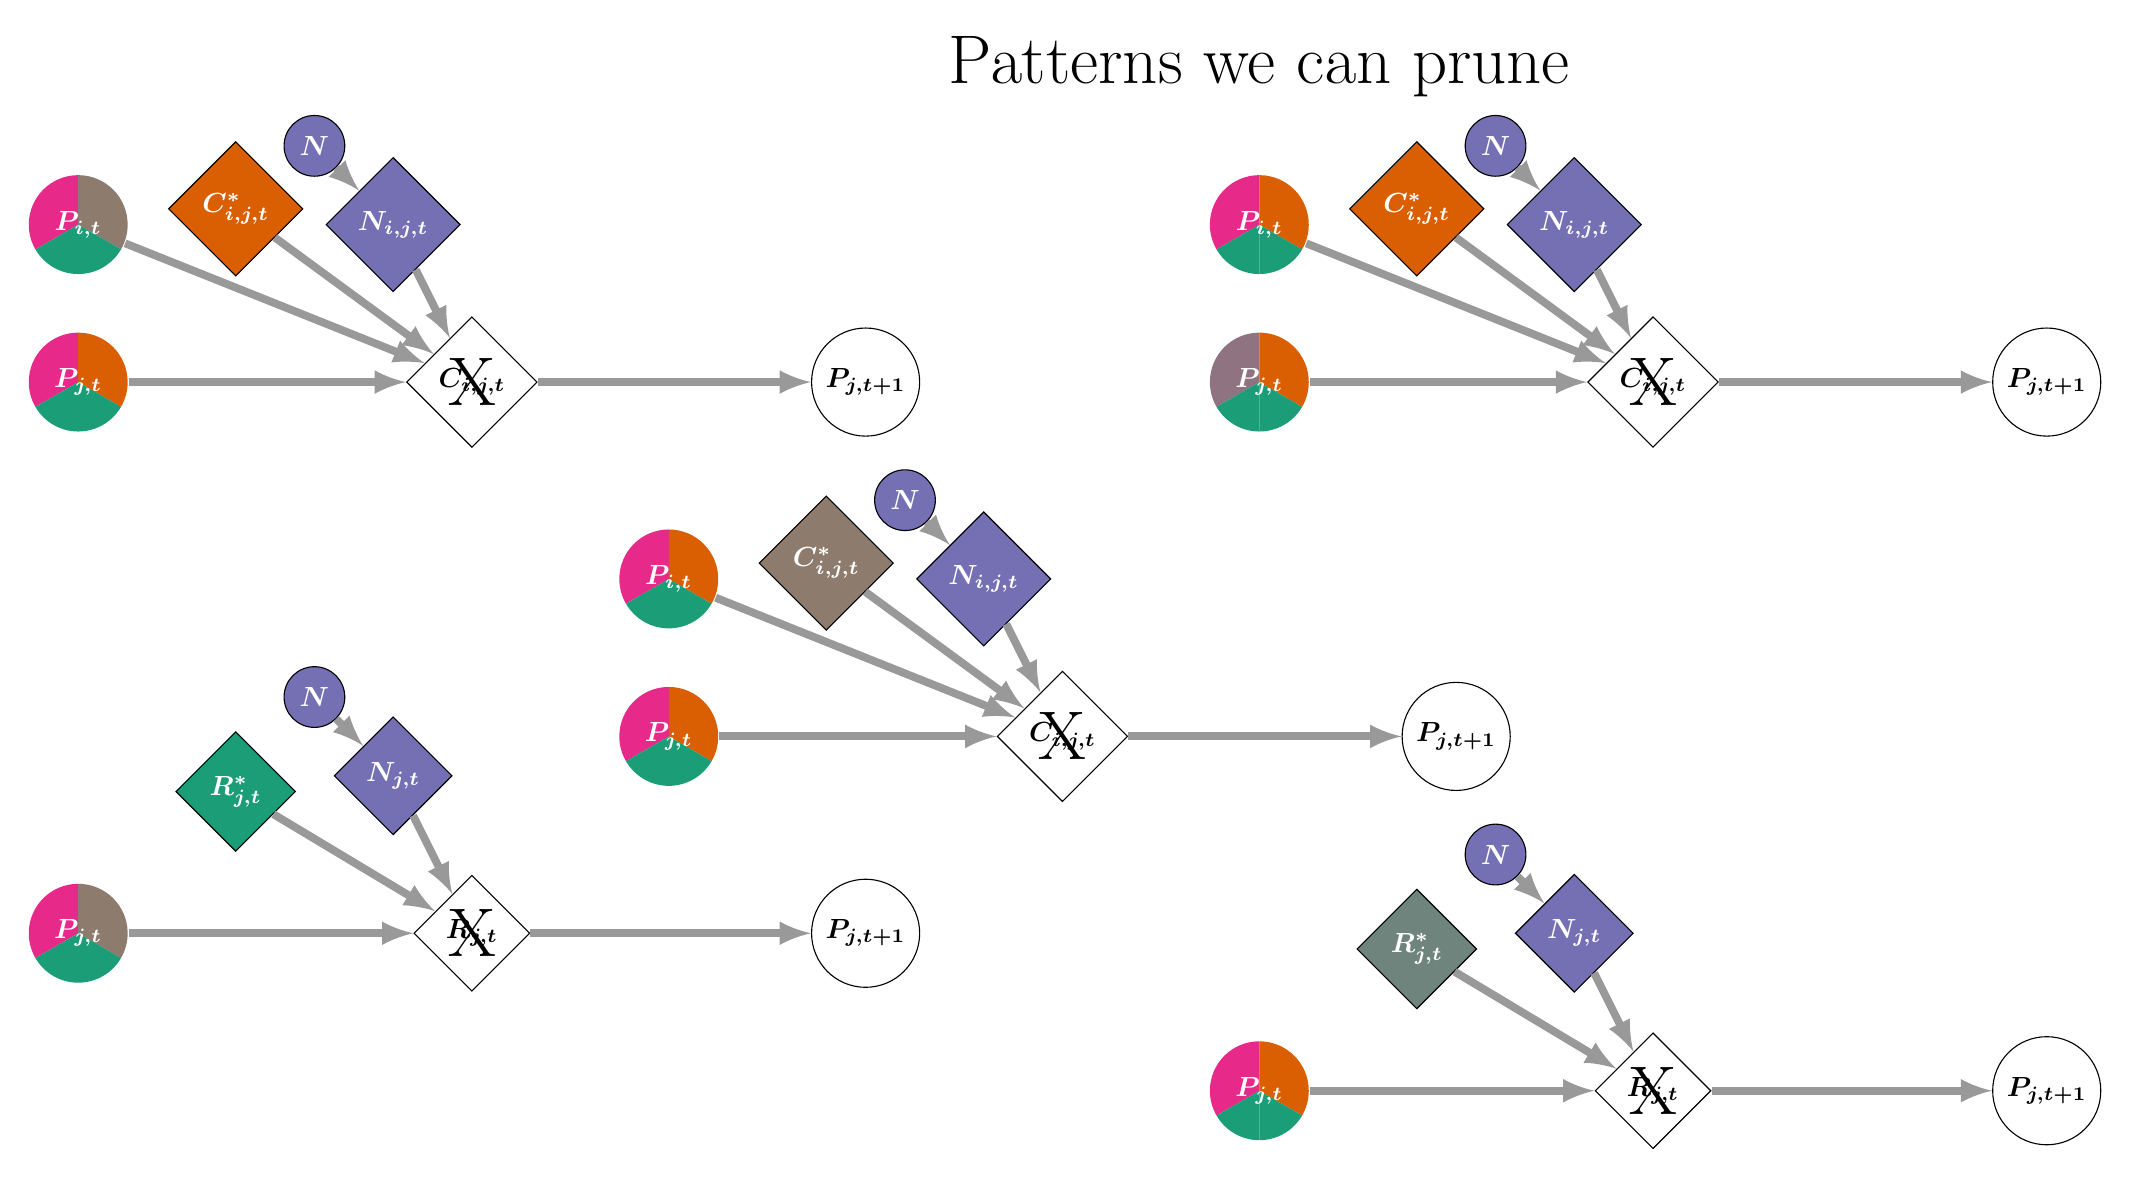
\begin{tikzpicture}
  \draw (0,4.5) node {\Huge Patterns we can prune};

  %% Infectious Contacts
  \draw (-10,0.5) node {\Leftscissors};
  \draw (-15,2.5) node[intervened node fill={susceptible,infection!15!gray,recovery},white] (P11) {$\bm{\bm{P_{i,t}}}$};
 % \draw (-15,2.5) node[node,fill=susceptible] (P11) {$\bm{\bm{P_{i,t}}}$};
  \draw (-15,0.5) node[intervened node fill={susceptible,infection,recovery},white] (P21) {$\bm{\bm{P_{j,t}}}$};
  \draw (-13,2.7) node[edge, contact] (E121) {$\bm{C^*_{i,j,t}}$};
  \draw (-12,3.5) node[circle,draw,intervention] (I) {$\bm{N}$};
  \draw (-11,2.5) node[edge, intervention] (I121) {$\bm{N_{i,j,t}}$};
  \draw (-5,0.5) node[node] (P22) {$\bm{P_{j,t+1}}$};
  \draw (-10,0.5) node[edge] (C121) {$\bm{C_{i,j,t}}$};
  
  \draw[-latex,color=black!40!white,line width=1mm] (P11) -- (C121);
  \draw[-latex,color=black!40!white,line width=1mm] (P21) -- (C121);
  \draw[-latex,color=black!40!white,line width=1mm] (C121) -- (P22);
  \draw[-latex,color=black!40!white,line width=1mm] (E121) -- (C121);
  \draw[-latex,color=black!40!white,line width=1mm] (I121) -- (C121);
  \draw[-latex,color=black!40!white,line width=1mm] (I) -- (I121);



    \draw (5,0.5) node {\Leftscissors};
  \draw (0,2.5) node[intervened node fill={susceptible,infection,recovery},white] (P11) {$\bm{\bm{P_{i,t}}}$};
 % \draw (-15,2.5) node[node,fill=susceptible] (P11) {$\bm{\bm{P_{i,t}}}$};
  \draw (0,0.5) node[intervened node fill={susceptible!15!gray,infection,recovery},white] (P21) {$\bm{\bm{P_{j,t}}}$};
  \draw (2,2.7) node[edge, contact] (E121) {$\bm{C^*_{i,j,t}}$};
  \draw (3,3.5) node[circle,draw,intervention] (I) {$\bm{N}$};
  \draw (4,2.5) node[edge, intervention] (I121) {$\bm{N_{i,j,t}}$};
  \draw (10,0.5) node[node] (P22) {$\bm{P_{j,t+1}}$};
  \draw (5,0.5) node[edge] (C121) {$\bm{C_{i,j,t}}$};
  
  \draw[-latex,color=black!40!white,line width=1mm] (P11) -- (C121);
  \draw[-latex,color=black!40!white,line width=1mm] (P21) -- (C121);
  \draw[-latex,color=black!40!white,line width=1mm] (C121) -- (P22);
  \draw[-latex,color=black!40!white,line width=1mm] (E121) -- (C121);
  \draw[-latex,color=black!40!white,line width=1mm] (I121) -- (C121);
  \draw[-latex,color=black!40!white,line width=1mm] (I) -- (I121);
  
  
  
      \draw (-2.5,-4) node {\Leftscissors};
  \draw (-7.5,-2) node[intervened node fill={susceptible,infection,recovery},white] (P11) {$\bm{\bm{P_{i,t}}}$};
 % \draw (-15,2.5) node[node,fill=susceptible] (P11) {$\bm{\bm{P_{i,t}}}$};
  \draw (-7.5,-4) node[intervened node fill={susceptible,infection,recovery},white] (P21) {$\bm{\bm{P_{j,t}}}$};
  \draw (-5.5,-1.8) node[edge, text=white,fill=infection!15!gray] (E121) {$\bm{C^*_{i,j,t}}$};
  \draw (-4.5,-1) node[circle,draw,intervention] (I) {$\bm{N}$};
  \draw (-3.5,-2) node[edge, intervention] (I121) {$\bm{N_{i,j,t}}$};
  \draw (2.5,-4) node[node] (P22) {$\bm{P_{j,t+1}}$};
  \draw (-2.5,-4) node[edge] (C121) {$\bm{C_{i,j,t}}$};
  
  \draw[-latex,color=black!40!white,line width=1mm] (P11) -- (C121);
  \draw[-latex,color=black!40!white,line width=1mm] (P21) -- (C121);
  \draw[-latex,color=black!40!white,line width=1mm] (C121) -- (P22);
  \draw[-latex,color=black!40!white,line width=1mm] (E121) -- (C121);
  \draw[-latex,color=black!40!white,line width=1mm] (I121) -- (C121);
  \draw[-latex,color=black!40!white,line width=1mm] (I) -- (I121);
  
  
    %% Recoveries
  \draw (-10,-6.5) node {\Leftscissors};
 % \draw (-15,2.5) node[node,fill=susceptible] (P11) {$\bm{\bm{P_{i,t}}}$};
  \draw (-15,-6.5) node[intervened node fill={susceptible,infection!15!gray,recovery},white] (P21) {$\bm{\bm{P_{j,t}}}$};
  \draw (-13,-4.7) node[edge, recovery] (E121) {$\bm{R^*_{j,t}}$};
  \draw (-12,-3.5) node[circle,draw,intervention] (I) {$\bm{N}$};
  \draw (-11,-4.5) node[edge, intervention] (I121) {$\bm{N_{j,t}}$};
  \draw (-5,-6.5) node[node] (P22) {$\bm{P_{j,t+1}}$};
  \draw (-10,-6.5) node[edge] (C121) {$\bm{R_{j,t}}$};
  
  \draw[-latex,color=black!40!white,line width=1mm] (P21) -- (C121);
  \draw[-latex,color=black!40!white,line width=1mm] (C121) -- (P22);
  \draw[-latex,color=black!40!white,line width=1mm] (E121) -- (C121);
  \draw[-latex,color=black!40!white,line width=1mm] (I121) -- (C121);
  \draw[-latex,color=black!40!white,line width=1mm] (I) -- (I121);



    \draw (5,-8.5) node {\Leftscissors};
 % \draw (-15,2.5) node[node,fill=susceptible] (P11) {$\bm{\bm{P_{i,t}}}$};
  \draw (0,-8.5) node[intervened node fill={susceptible,infection,recovery},white] (P21) {$\bm{\bm{P_{j,t}}}$};
  \draw (2,-6.7) node[edge, fill=recovery!15!gray,text=white] (E121) {$\bm{R^*_{j,t}}$};
  \draw (3,-5.5) node[circle,draw,intervention] (I) {$\bm{N}$};
  \draw (4,-6.5) node[edge, intervention] (I121) {$\bm{N_{j,t}}$};
  \draw (10,-8.5) node[node] (P22) {$\bm{P_{j,t+1}}$};
  \draw (5,-8.5) node[edge] (C121) {$\bm{R_{j,t}}$};
  
  \draw[-latex,color=black!40!white,line width=1mm] (P21) -- (C121);
  \draw[-latex,color=black!40!white,line width=1mm] (C121) -- (P22);
  \draw[-latex,color=black!40!white,line width=1mm] (E121) -- (C121);
  \draw[-latex,color=black!40!white,line width=1mm] (I121) -- (C121);
  \draw[-latex,color=black!40!white,line width=1mm] (I) -- (I121);
  
\end{tikzpicture}


\end{document}

  %% Recovery
  \draw (0,0.5) node[node] (P21) {$\bm{P_{j,t}}$};
  \draw (2,2.7) node[edge, recovery] (E121) {$\bm{R^*_{j,t}}$};
  \draw (3,3.5) node[node, intervention] (I) {$\bm{N}$};
  \draw (4,2.5) node[edge, intervention] (I11) {$\bm{N_{j,t}}$};
  \draw (10,0.5) node[node] (P22) {$\bm{P_{j,t+1}}$};
  \draw (5,0.5) node[ edge] (R121) {$\bm{R_{j,t}}$};
  
  \draw[-latex,color=black!40!white,line width=1mm] (P21) -- (R121);
  \draw[-latex,color=black!40!white,line width=1mm] (R121) -- (P22);
  \draw[-latex,color=black!40!white,line width=1mm] (E121) -- (R121);
  \draw[-latex,color=black!40!white,line width=1mm] (I11) -- (R121);
  \draw[-latex,color=black!40!white,line width=1mm] (I) -- (I11);
